\chapter{Theoretical Background}
\label{sec:theoretical_background}

%-------------------------------------------------------------------
\section{Robotics and Object Handling}
\label{subsec:robotics_and_handling}

\subsection{Robotics}
\label{subsubsec:robotics}

An industrial robot is an automatically controlled, reprogrammable multipurpose manipulator(s), programmable in
three or more axes, which can be either fixed in place or fixed to a mobile platform for use
in automation applications in an industrial environment~\cite{Lee2022Vocabulary}. A typical robotic system consists of a kinematic chain of rigid links
connected by actuated joints, a set of sensors, a controller and an end-effector mounted at the flange of the last link. The configuration of the
manipulator is described by its joint variables, while the position and orientation of the end-effector are described in a Cartesian task
space~\cite{Malik2022A}. The mapping between these two spaces is established through forward and inverse kinematics, which form the basis for
trajectory planning and motion control~\cite{Singh2022Kinematics}.

Modern manufacturing systems increasingly require flexibility to accommodate
changing production demands, mass customization, increasing product variants,
and decreasing batch sizes~\cite{Wiese2022Flexible,Bilancia2023An}. Robot-cell
reconfiguration and programming nevertheless remain time-consuming and often
require specialist expertise~\cite{Wiese2022Flexible}. Task-specific assets such
as grippers, sensors, and actuators provide robot cells with the capabilities
required for particular manufacturing tasks~\cite{Wiese2022Flexible}.

% \subsubsection{Handling of Objects using Grippers}
% \label{subsubsec:handling_with_grippers}

% Object handling denotes the sequence of establishing, maintaining and releasing a mechanical connection between an end-effector and a workpiece. The
% component responsible for this connection is the gripper, which can be classified by the physical principle used to transmit
% forces~\cite{Zhou2021Bio-Inspired}. Impactive grippers, such as parallel-jaw and multi-finger designs, grasp objects through direct mechanical contact,
% relying on contact forces and friction to maintain the grasp~\cite{Zhou2021Bio-Inspired}. Astrictive grippers, most prominently vacuum-based suction
% systems, rely on a pressure difference acting on a sealed contact area. Further principles include magnetic and electroadhesive as well as contigutive
% approaches based on adhesion~\cite{Zhou2021Bio-Inspired}.

% The selection and design of a gripper is governed by the properties of the workpiece and the process. Relevant criteria include the mass and the
% inertia of the object, the accessible contact surfaces, surface roughness and porosity, geometric tolerances, the required positioning accuracy, cycle
% time, etc. ~\cite{Ivanov2024New, Morecki1999Manipulator}. Since these criteria interact, gripper design is inherently a trade-off
% problem~\cite{Cramer2022Development}. A gripper that is optimally adapted to a single workpiece is often unsuitable for others, whereas a gripper
% intended for a family of workpieces must compromise between competing geometric requirements~\cite{Lundstrom1974Industrial,Hota2024Automated}. This
% tension between specialisation and generalisation is the central motivation for treating gripper configuration as a multi-objective optimisation
% problem~\cite{Mnyussiwalla2022Evaluation}.

\subsection{Bin Picking Problem}
\label{subsubsec:bin_picking}

Bin picking describes the task of removing individual workpieces from an unordered accumulation of parts, typically supplied in a container, and
transferring them to a defined target pose~\cite{Khalid2021Automatic,Kyprianou2023Bin-Picking}. The task combines perception, grasp planning,
collision-free motion planning and physical grasp execution. Because the parts are randomly oriented and may be partially occluded or entangled, the
pose of the next object to be grasped is not known in advance and must be estimated from sensor data at runtime~\cite{Zhang2021A,Tipary2021Planning}.

For gripper design, the decisive consequence of this setting is that a grasp cannot be planned for one privileged object
pose~\cite{Khalid2021Automatic}. The gripper must be able to reach and hold the workpiece across a broad range of orientations and partial
accessibility conditions, which implies that a useful gripper configuration provides several alternative grasp candidates distributed over the object
surface rather than one single optimal contact~\cite{Khalid2021Automatic,Wan2020Planning}. Additional constraints arise from the confined working space
inside the bin, where collisions between the gripper body and the bin walls or neighboring parts restrict the set of feasible approach
directions~\cite{Tipary2021Planning,Spenrath2012Gripping}. These requirements directly motivate the objectives used in this thesis, in particular the
diversity of the available grasps for the suction cup gripper and the geometric conformance of the finger contour for the two-finger gripper.

%-------------------------------------------------------------------
\section{Gripper Theory and Geometric Representation}
\label{subsec:gripper_theory}

\subsection{Grasp Theory}
\label{subsubsec:grasp_theory}

A grasp is a configuration of contact points between a gripper and a workpiece such that the gripper can resist external forces and torques applied to
the object~\cite{Prattichizzo2014Robot}. The classical criterion for grasp quality is \emph{force closure}. A grasp is force-closed if the contact
forces available at the contact points can produce any net wrench on the object, meaning that arbitrary disturbances can be
resisted~\cite{Nguyen1986Constructing}. Force closure requires a sufficient number of contacts with appropriate friction properties and geometric
placement.
\begin{figure}[H]
    \centering
    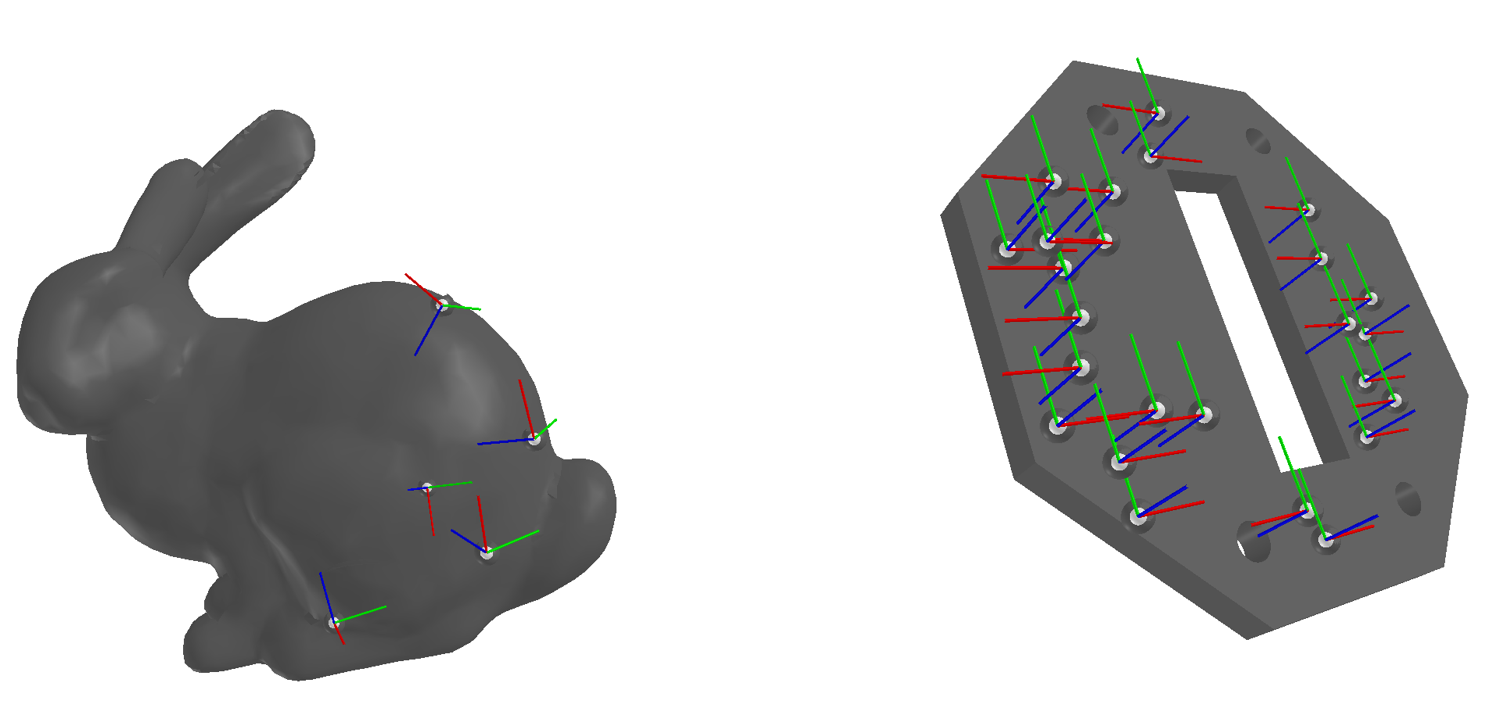
\includegraphics[width=0.8\textwidth]{fig/th_bg/grasps.png}
    \caption{Visualization of a grasp configuration on workpieces.}
    \label{fig:grasp}
\end{figure}
Figure~\ref{fig:grasp} illustrates grasp configurations for two workpieces: the
Stanford Bunny and the IPA Intermediate Plate. Each point on the workpiece
surface encodes the translation and rotation required to transform the gripper's
Tool Center Point (TCP) from its initial pose to the corresponding grasp pose.

\subsection{Suction Cup Grippers}
\label{subsubsec:suction_cup_grippers}

Suction cup grippers belong to the astrictive gripper class and generate holding force from a pressure difference between the evacuated volume inside
the cup and the ambient atmosphere. The holding force is defined as:

\begin{equation}
    \begin{gathered}
        F_{\mathrm{hold}} = \frac{\Delta p \cdot A_{\mathrm{seal}}}{S}, \\[4pt]
        \Delta p \in \left(0,\, p_{\mathrm{atm}}\right] \subset \mathbb{R}_{>0},\quad
        A_{\mathrm{seal}} \in \mathbb{R}_{>0},\quad
        S \in \left[1,\, \infty\right) \subset \mathbb{R},\quad
        F_{\mathrm{hold}} \in \mathbb{R}_{>0}
    \end{gathered}
\end{equation}

where $\Delta p$ is the pressure difference between the evacuated cup volume and the ambient atmosphere, bounded above by the atmospheric pressure
$p_{\mathrm{atm}}$ since a perfect vacuum cannot be exceeded, $A_{\mathrm{seal}}$ is the effective sealed area enclosed by the cup lip, and $S \geq 1$
is a safety factor accounting for acceleration, orientation and friction conditions~\cite{Zhou2021Bio-Inspired,Gabriel2020Modeling}. The holding force
is strictly positive for any non-vanishing pressure difference acting on a non-degenerate sealed area. The decisive requirement is therefore an
airtight seal between the cup lip and the workpiece surface, which restricts applicable surfaces to regions that are sufficiently smooth, non-porous
and locally flat or only moderately curved relative to the compliance of the cup.

Practical implementations frequently use several cups arranged on a common mounting plate. Distributing the load over multiple cups increases the
total holding force, provides redundancy if individual cups fail to seal, and, most importantly for handling, generates a resistance to tilting
moments~\cite{Mantriota_2007}. The moment capacity depends on the spatial arrangement of the active cups, which
is commonly characterized through the area of the polygon or triangle spanned by the sealing contacts~\cite{Gabriel2020Modeling}. A large spanned area
yields a stable grasp, whereas narrowly clustered cups behave similarly to a single contact. The placement of the cups on the mounting plate is thus
the central design variable, and it must be chosen such that valid sealing contacts are achievable on every workpiece of the considered family.\cite{Roa_Suarez_2015}

\subsection{Multi-Finger Grippers}
\label{subsubsec:multi_finger_grippers}

Multi-finger grippers are impactive grippers that transmit forces through direct contact between movable jaws and the workpiece. They are classified
by the number of fingers, the kinematics of the jaw motion and the number of actuated degrees of freedom~\cite{Khalid2025Design}. Two-finger parallel
grippers with a single actuator represent the industrial standard because of their mechanical simplicity, robustness and low control
effort~\cite{Ciocarlie2014The}. Three-finger centric designs provide self-centring behavior for rotationally symmetric parts, while anthropomorphic
hands with many degrees of freedom offer high versatility at the cost of complexity~\cite{Simionescu2008Mathematical,Backus2016An}.

Two grasp modes are commonly distinguished. Force-closure grasps hold the object through friction at the contact surfaces and therefore depend on the
applied clamping force and the friction coefficient. Form-closure grasps immobilize the object through the geometry of the contacts alone, so that no
disturbance can move the object without deformation~\cite{Bicchi1995On}. Because a mechanically simple gripper provides few actuated degrees of
freedom, the ability to realize form closure is shifted from the kinematics to the geometry of the jaws. This is the reason why application-specific
jaw inserts, frequently produced additively, are widely used in industry and why the jaw contour is the natural design variable for
optimization.~\cite{Gebauer2024Uncertainty-integrating}


%-------------------------------------------------------------------
\section{Optimization Theory}
\label{subsec:optimization_theory}

\subsection{Black-Box Optimization}
\label{subsubsec:black_box_optimization}

A black-box optimization problem is one in which the objective function has no known analytical form and no gradient information is available to the
optimizer~\cite{Audet2017Derivative-Free}. The function can only be queried at candidate input points, returning a scalar or vector output. This
setting arises naturally in engineering design when objectives are evaluated through computationally expensive procedures, making gradient computation
either impossible or impractical. Because each function evaluation may be costly, black-box optimizers must find high-quality solutions within a
limited evaluation budget, placing emphasis on sample efficiency.~\cite{xu2023constrained,Paulson2021COBALT}

\subsection{Multi-Objective Optimization}
\label{subsubsec:multi_objective_optimization}

Multi-objective optimization (MOO) refers to the simultaneous optimization of two or more conflicting objective functions over a shared decision
space~\cite{Deb2011Multi-objective}. Formally, a multi-objective minimization problem is defined as

\begin{equation}
    \label{eq:moop}
    \begin{gathered}
        \min_{\mathbf{x} \in \mathcal{X}} \mathbf{f}(\mathbf{x}) =
        \bigl(f_1(\mathbf{x}),\, f_2(\mathbf{x}),\, \ldots,\, f_k(\mathbf{x})\bigr),
        \\[4pt]
        \mathcal{X} \subseteq \mathbb{R}^{d},
        \quad
        d \in \left\{ n \in \mathbb{Z} \mid n \ge 1 \right\},
        \quad
        k \in \left\{ n \in \mathbb{Z} \mid n \ge 2 \right\},
        \\[4pt]
        f_i : \mathcal{X} \rightarrow \mathbb{R},
        \quad
        \forall\, i \in \{1,\ldots,k\},
        \qquad
        \mathbf{f}(\mathbf{x}) \in \mathbb{R}^{k},
        \quad
        \forall\, \mathbf{x} \in \mathcal{X}.
    \end{gathered}
\end{equation}

In Eq.~\ref{eq:moop}, $\mathbf{x}$ is the decision variable vector, $\mathcal{X}$ is the feasible decision space, and $k \geq 2$ is the number of objectives. When
objectives conflict, no single solution minimizes all objectives simultaneously. Instead, a set of trade-off solutions exists, collectively forming
the Pareto front. The goal of a multi-objective optimizer is therefore not to find a single best solution but to approximate this trade-off surface as
accurately and completely as possible~\cite{Deb2011Multi-objective,Gunantara2018A}.

\subsection{Pareto Optimality}
\label{subsubsec:pareto_optimality}

The concept of Pareto optimality provides the theoretical foundation for comparing solutions in a multi-objective setting. A solution
$\mathbf{x}^{(a)}$ is said to \emph{dominate} $\mathbf{x}^{(b)}$, written $\mathbf{x}^{(a)} \prec \mathbf{x}^{(b)}$, if and only if

\begin{equation}
    \label{eq:pareto_dominance}
    \begin{gathered}
        f_i(\mathbf{x}^{(a)}) \leq f_i(\mathbf{x}^{(b)}) \quad \forall\, i \in \{1,\ldots,k\}
        \quad \text{and} \quad
        \exists\, j \in \{1,\ldots,k\} : f_j(\mathbf{x}^{(a)}) < f_j(\mathbf{x}^{(b)}),
        \\[4pt]
        \mathbf{x}^{(a)},\, \mathbf{x}^{(b)} \in \mathcal{X},
        \quad
        \mathbf{f} = (f_1,\ldots,f_k) : \mathcal{X} \rightarrow \mathbb{R}^{k},
        \quad
        k \in \left\{ n \in \mathbb{Z} \mid n \ge 2 \right\}.
    \end{gathered}
\end{equation}

A solution is called \emph{Pareto optimal} if no other feasible solution dominates it. The set of all Pareto-optimal solutions in the decision space
is the \emph{Pareto set}, and its image in the objective space is the \emph{Pareto front}. In practice, algorithms compute an approximation of the
Pareto front, and the quality of this approximation is assessed using performance indicators such as the hypervolume
indicator.~\cite{Audet2018Performance,Shang2021A}

\begin{figure}[H]
    \centering
    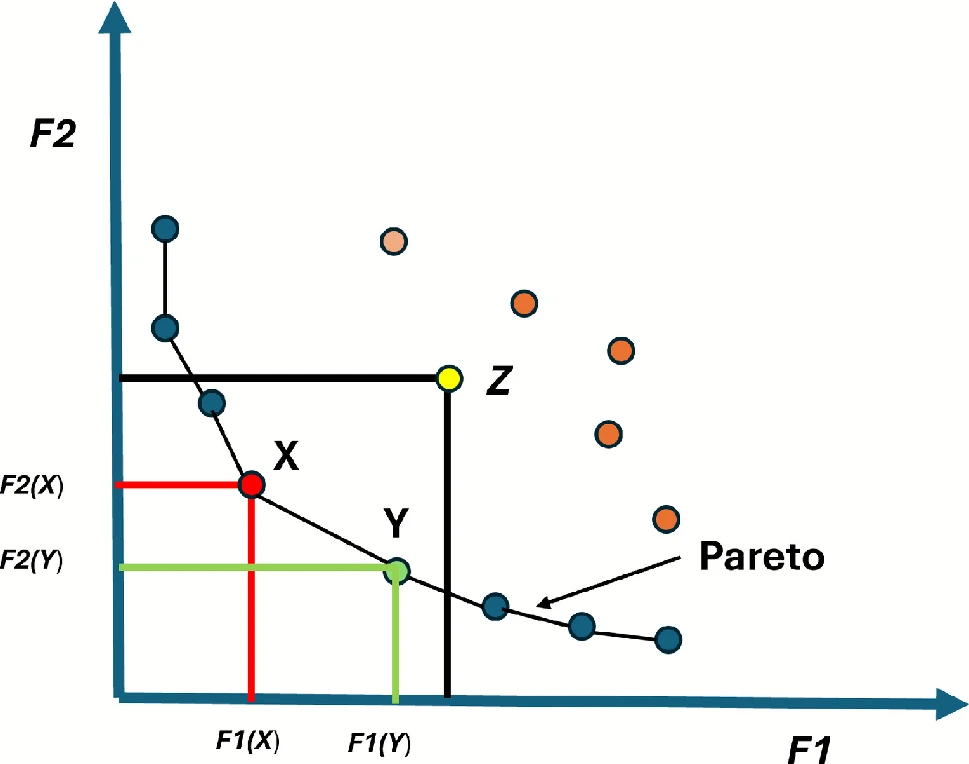
\includegraphics[width=0.6\textwidth]{fig/th_bg/pareto_front.png}
    \caption{Example of a Pareto Front.~\cite{Tarunika2026}}
    \label{fig:pareto_front}
\end{figure}

Figure~\ref{fig:pareto_front} illustrates the concept of dominated and non-dominated solutions in a multi-objective optimization problem (MOP) with
two objectives. The objective is to minimize both objective functions. The connected curve represents the Pareto front (PF), which includes all
Pareto-optimal solutions. Solution $X_2$ has higher values for both $f_1$ and $f_2$ when compared to solutions $X_1$ and $Y$. Thus, solutions $X_1$
and $Y$ dominate solution $X_2$. However, since neither $X_1$ nor $Y$ dominates the other, they are considered non-dominated solutions~\cite{Tarunika2026}.


\subsection{Many-Objective Optimization}
\label{subsubsec:many_objective_optimization}

Problems with four or more objectives are commonly referred to as many-objective optimization problems~\cite{Li2015Many-Objective}. As the number of
objectives grows, the proportion of mutually non-dominated solutions in a randomly sampled population increases rapidly, an effect known as dominance
resistance. Pareto dominance then loses its ability to discriminate between candidates, so selection pressure towards the Pareto front deteriorates
and the search degenerates into an essentially random walk guided mainly by diversity preservation.~\cite{Li2015Many-Objective,VonLuecken2014A}

The number of solutions required to cover a $k$-dimensional front grows exponentially with $k$, visual inspection of the approximation set becomes
impractical, and the computation of indicators such as the hypervolume becomes expensive~\cite{Guerreiro2020}. Algorithm design responds to these
issues either by replacing dominance with decomposition into scalar subproblems, by introducing reference points or reference directions to structure
the objective space, or by using an indicator as the selection criterion~\cite{Li2015Many-Objective,das_dennis}.

\subsection{No Free Lunch Theory}
\label{subsubsec:no_free_lunch}

The No Free Lunch (NFL) theorems for optimization state that, averaged over the set of all possible objective functions, all non-repeating search
algorithms exhibit identical expected performance~\cite{Adam2019No, Wolpert1997No}. Any advantage that an algorithm demonstrates on one class of
problems is therefore compensated by a corresponding disadvantage on another class. Corresponding results have been derived for the multi-objective
case.~\cite{Wolpert1997No, Haftka2016Requirements}

The practical consequence is that there is no universally superior optimization algorithm and that the question of which algorithm to use is only
meaningful with respect to a specific problem class~\cite{Cotta1998A}. This provides the methodological justification for the empirical approach taken
in this thesis. Rather than seeking a generally best algorithm, the objective is to determine which algorithms perform well on the particular
structure of gripper configuration problems, and how sensitive this ranking is to workpiece geometry and to the dimensionality of the objective space~\cite{Doerterler2021Analyzing}.

\subsection{Evolutionary Algorithms}
\label{subsubsec:evolutionary_algorithms}

Evolutionary algorithms (EAs) are a family of population-based metaheuristics inspired by the principles of biological evolution~\cite{Cheng2018Modelbased}. A population of
candidate solutions is maintained across discrete generations. At each generation, new candidate solutions are generated through variation operators,
typically crossover, which recombines pairs of existing solutions, and mutation, which introduces random perturbations, and a selection mechanism
retains the most promising individuals for the next generation based on their objective values~\cite{Slowik2020Evolutionary}. This loop continues until a termination criterion is
met, such as a maximum number of function evaluations or convergence of the population~\cite{Abulail2025Enhanced}.

\begin{figure}[H]
    \centering
    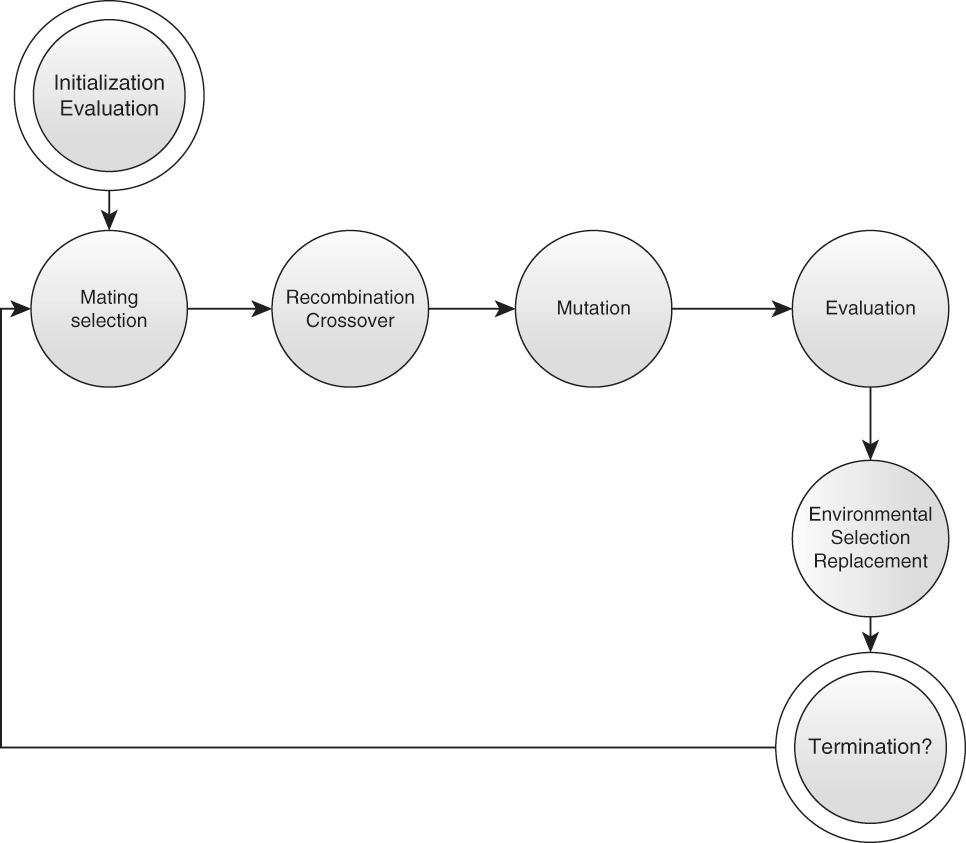
\includegraphics[width=0.8\textwidth]{fig/th_bg/Evolutionary_flowchart.png}
    \caption{The evolutionary cycle, basic working scheme of all EAs~\cite{Evolutionary_Algos}.}
    \label{fig:evolutionary_flowchart}
\end{figure}

Figure~\ref{fig:evolutionary_flowchart} shows the basic working scheme shared by all EAs. After
initialization and evaluation of the initial population, the algorithm iteratively
applies mating selection, recombination (crossover), mutation, evaluation of the
offspring, and environmental selection (replacement), until a termination criterion
is satisfied. The individual steps of this cycle can be described as follows.

\subsubsection{Initialization and Evaluation}
The algorithm begins by creating a population of candidate solutions.
Random initialization is a simple and commonly used approach, although
problem-specific methods can also be employed, for example by including
known good solutions as starting points. Each individual is then evaluated
to obtain a measure of its quality, referred to as its fitness. When the
underlying problem is an optimization problem, this evaluation is performed
using the objective function. The evaluated population provides the starting
point for the subsequent variation and selection steps.
~\cite{Evolutionary_Algos}

\subsubsection{Mating Selection}
Mating selection chooses individuals from the current population to act
as parents for offspring generation. Selection introduces a bias toward
individuals with better fitness. In genetic algorithms, one possible
method is fitness-proportional selection, in which selection probabilities
depend on individual fitness values. Another method is tournament
selection, in which a small set of individuals is sampled randomly, their fitness
values are compared, and the best individual in that set is selected.
Thus, in the tournament procedure described here, randomness enters
through the choice of participants, while the winner is determined by
their fitness.
~\cite{Evolutionary_Algos}

\subsubsection{Recombination (Crossover)}
Recombination, also called crossover, generates offspring by combining
information from two or more parents. It rearranges information already
present in the population and can combine favorable characteristics from
different individuals. The specific operator depends on the representation
of the candidate solutions. For binary strings, examples include one-point,
two-point, and uniform crossover. In one-point crossover, a crossover
position is chosen randomly and segments of two parent strings are
exchanged. Recombination is used in several evolutionary algorithm
families, but it is not a component of evolutionary programming.
~\cite{Evolutionary_Algos}

\subsubsection{Mutation}
Mutation is a stochastic variation operator that modifies an individual
and introduces new information into the population. Unlike recombination,
which rearranges existing information, mutation can explore regions of
the search space not currently covered by the population. Its implementation
depends on the representation: binary mutation can flip a randomly chosen
bit, whereas evolution strategies can perturb real-valued variables using
Gaussian mutations. In evolution strategies, strategy parameters such as
the mutation step size influence the operator and can themselves be
adapted during the search.
~\cite{Evolutionary_Algos}

\subsubsection{Evaluation of the Offspring}
After variation, the offspring are evaluated to determine their fitness
before replacement or survivor selection is performed. This follows the
same evaluation principle used for the initial population. In applications
where fitness evaluation requires a time-consuming numerical model or
physical experiment, evaluating candidate solutions can be expensive.
~\cite{Evolutionary_Algos}

\subsubsection{Environmental Selection (Replacement)}
Environmental selection determines which individuals survive into the
next population. The replacement procedure depends on the algorithm.
For example, the evolutionary programming scheme may combine parents and offspring before selecting survivors to
keep the population size constant. In contrast, a genetic algorithm may
replace the parental population with offspring independently of fitness.
For multi-objective optimization, selection requires a ranking mechanism
that accounts for several objectives. NSGA-II uses non-dominated ranking
and crowding distance, whereas SMS-EMOA uses marginal hypervolume
contributions.
~\cite{Evolutionary_Algos}

\subsubsection{Termination}
After environmental selection, a termination criterion is checked. If it is not
satisfied, the cycle continues with the mating selection of the next generation, otherwise the
current population, or the non-dominated subset of all evaluated solutions is returned as the
result.
~\cite{Evolutionary_Algos}

EAs are well suited to black-box multi-objective optimization because they require no gradient information, naturally maintain a diverse population of
trade-off solutions, and are robust to noisy or discontinuous objective landscapes~\cite{Zheng2022An}. Multi-objective evolutionary algorithms (MOEAs) extend the basic
EA framework with selection mechanisms based on Pareto dominance or decomposition, enabling them to approximate the Pareto front in a single
run.~\cite{Ishibuchi2017Performance,Li2015An}

\subsection{Bayesian Optimization}
\label{subsubsec:bayesian_optimization}

Bayesian optimization (BO) is a sequential model-based strategy for the global optimization of expensive black-box functions~\cite{Lu2022Surrogate}. A probabilistic
surrogate model, most commonly a Gaussian process (GP), is fitted to the observations collected so far~\cite{Frazier2018A}. The surrogate provides both
a mean prediction and an uncertainty estimate at unobserved locations, which together define an \emph{acquisition function} that balances exploration
of uncertain regions with exploitation of promising ones~\cite{Frazier2018A,Candelieri2021A}. The point that maximizes the acquisition function is
selected as the next evaluation, after which the surrogate is updated and the process repeats~\cite{Wang2022Recent, olson2025ax}. Because the
surrogate concentrates the sampling effort on informative regions, BO typically requires far fewer function evaluations than population-based methods,
which makes it attractive whenever the evaluation budget is the limiting factor~\cite{Wang2022Recent}.

\subsubsection{Gaussian Process Surrogates}
A Gaussian process defines a distribution over functions and is fully specified by a mean
function $m(\mathbf{x})$ and a positive semi-definite covariance or kernel function
$\kappa(\mathbf{x}, \mathbf{x}')$, written as
$f(\mathbf{x}) \sim \mathcal{GP}\bigl(m(\mathbf{x}),\, \kappa(\mathbf{x}, \mathbf{x}')\bigr)$~\cite{Schulz2016A}.
Conditioning the prior on the observed data set
$\mathcal{D} = \{(\mathbf{x}_i, y_i)\}_{i=1}^{n_{\mathrm{obs}}}$, where $y_i \in \mathbb{R}$
is the response measured at $\mathbf{x}_i$ and $n_{\mathrm{obs}}$ the number of
evaluations performed so far, yields a posterior that is again Gaussian, with closed-form
predictive mean $\mu(\mathbf{x})$ and non-negative predictive variance
$\sigma^2(\mathbf{x})$ at any query point~\cite{Park_2022_RobustGP}. The kernel encodes the
assumed smoothness and length scale of the underlying function, with the Mat\'ern and squared exponential kernels being the most common choices, and its
hyperparameters are estimated by maximizing the marginal likelihood~\cite{Kouw_2025_BayesianAutoregression}. An additional noise term accounts for stochastic or
numerically imprecise evaluations~\cite{Binois2021A}. The main limitations of GP surrogates are the cubic scaling of exact inference with the number of
observations and a loss of predictive quality in high-dimensional decision spaces~\cite{Frazier2018A}.

\begin{figure}[H]
    \centering
    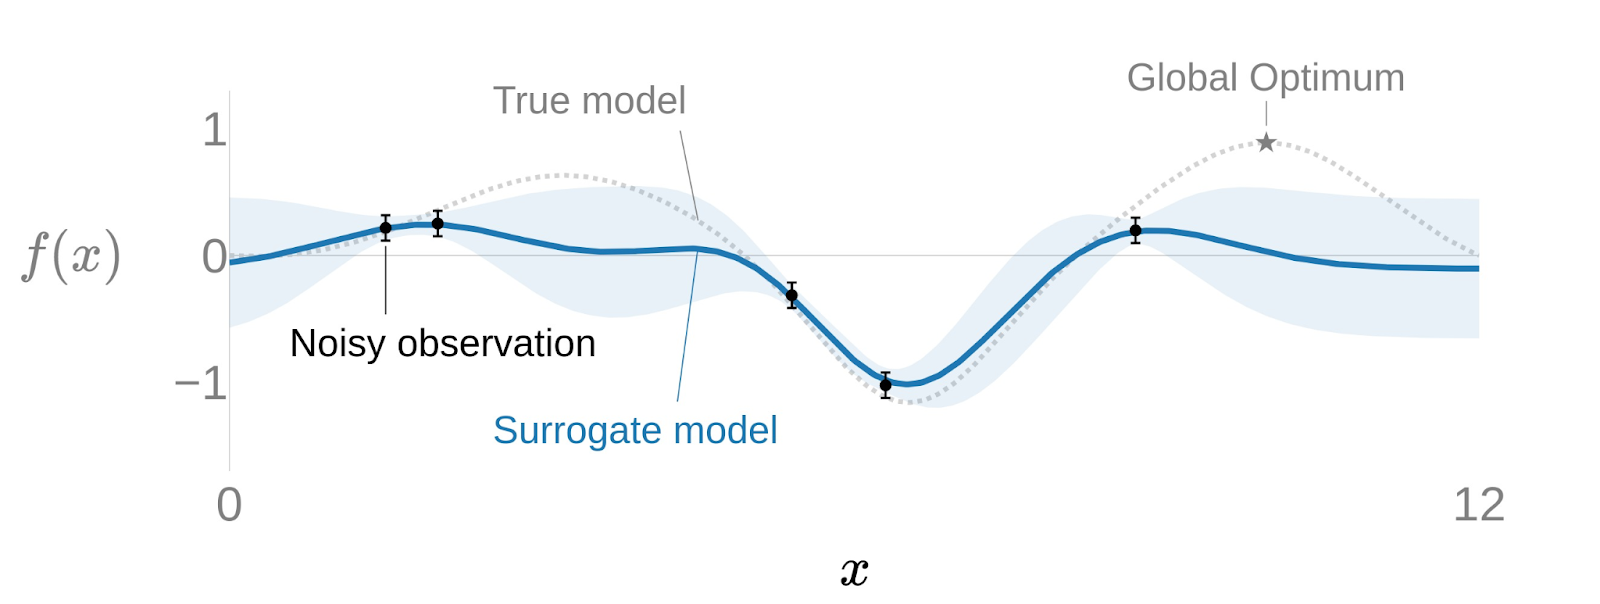
\includegraphics[width=0.8\textwidth]{fig/th_bg/SurrogateModel.png}
    \caption{Surrogate Model~\cite{olson2025ax}.}
    \label{fig:surrogate_model}
\end{figure}

In Figure~\ref{fig:surrogate_model} a surrogate model is fit to five noisy observations using a GP to predict the objective, depicted by the solid line,
and uncertainty estimates, illustrated by the width of the shaded bands. This objective is predicted for the entire range of possible parameter
values, corresponding to the full x-axis. Importantly, the model is able to predict the outcome and quantify the uncertainty of configurations that
have not yet been tested. Intuitively, the uncertainty bands are tight in regions that are well-explored and become wider as we move away from them.~\cite{olson2025ax}



\subsubsection{Acquisition Functions}
The acquisition function converts the posterior of the surrogate into a scalar utility that quantifies how promising a candidate point is. Expected
improvement (EI) measures the expected amount by which a candidate improves on the best observed value,

\begin{equation}
    \begin{gathered}
        \alpha_{\mathrm{EI}}(\mathbf{x}) =
        \mathbb{E}\bigl[\max\bigl(f_{\min} - f(\mathbf{x}),\, 0\bigr)\bigr], \\[4pt]
        \mathbf{x} \in \mathcal{X} \subseteq \mathbb{R}^{d},\quad
        f_{\min} = \min_{i \in \{1,\ldots,n_{\mathrm{obs}}\}} y_i \in \mathbb{R},\quad
        \alpha_{\mathrm{EI}} : \mathcal{X} \rightarrow \mathbb{R}_{\geq 0}
    \end{gathered}
\end{equation}

where $\mathbb{E}[\cdot]$ denotes the expectation taken with respect to the posterior of
the surrogate at $\mathbf{x}$ and $f_{\min}$ is the best objective value observed so far.
Truncating the improvement at zero renders the acquisition non-negative, so that
candidates which are not expected to improve on the incumbent receive zero utility. The
expression admits a closed form for a Gaussian posterior.~\cite{Binois2021A, olson2025ax}

\begin{figure}[H]
    \centering
    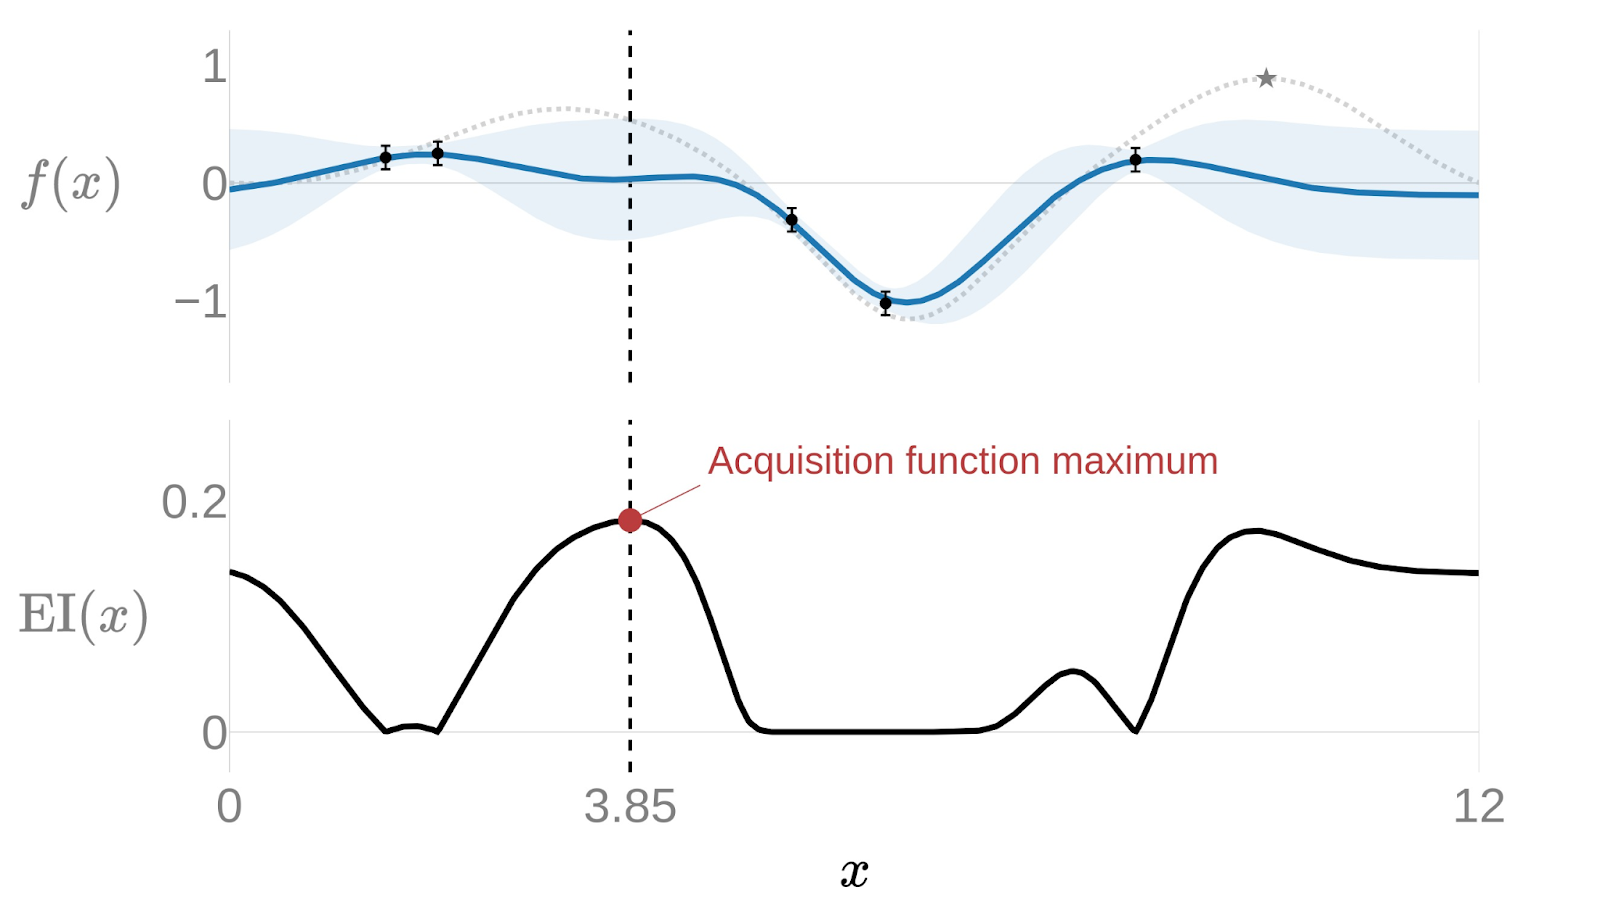
\includegraphics[width=0.8\textwidth]{fig/th_bg/acquisition_fn.png}
    \caption{Acquisition Function~\cite{olson2025ax}.}
    \label{fig:acquisition_fn}
\end{figure}

A visualization of the expected improvement based on the surrogate model predictions is shown in Figure~\ref{fig:acquisition_fn}, where the next
suggestion is where the expected improvement is at its maximum. Once a new highest EI is selected and evaluated, the surrogate model is retrained and a new suggestion
is made. This process continues iteratively until a stopping condition, set by the user, is reached.~\cite{olson2025ax}

\subsubsection{Multi-Objective Bayesian Optimization}
\label{subsec:bayesian_moo}

Multi-objective Bayesian optimization extends Bayesian optimization
to problems with several competing objectives. Surrogate models
predict objective values and their uncertainty, while an acquisition
function guides the selection of new candidates. The aim is to
approximate a set of Pareto-optimal trade-offs rather than identify a
single optimum~\cite{Daulton2021qNEHVI}.

Different acquisition strategies address this task in different ways.
Scalarization combines the objectives into a scalar utility and can
explore different trade-off regions by varying the scalarization
parameters. Hypervolume-based methods assess candidates according to
their expected contribution to the dominated objective-space volume
~\cite{Daulton2021qNEHVI}. Information-theoretic methods instead seek
candidates expected to provide information about the Pareto
front~\cite{Tu2022Joint}.

Before model-based candidate selection, initial observations can be
obtained using a space-filling experimental design
~\cite{Frazier2018A}. For bounded continuous variables, one possible
starting point is the center of the search space, given by the midpoint
of each variable's interval. Additional points can be generated using
a Sobol sequence. Sobol sequences are low-discrepancy sequences
designed to distribute points across a bounded space.~\cite{Sobol1967}

A Gaussian process can be used to model an individual objective, and
separate models can be fitted to multiple objectives
~\cite{Daulton2021qNEHVI}. The covariance kernel specifies how
function values at different inputs are related. For example, the
radial basis function (RBF) kernel assigns greater correlation to
nearby points. Its length-scale parameters control how quickly that
correlation decreases with distance, expressing an assumption of a
smooth objective function~\cite{Frazier2018A}.

Expected hypervolume improvement measures the expected increase in
dominated hypervolume relative to a reference point. Its noisy,
batch-capable extension, qNEHVI (q-Noisy Expected Hypervolume Improvement), accounts for uncertainty about the
objective values at previously evaluated points and can assess a set
of candidates jointly~\cite{Daulton2021qNEHVI}. The related
qLogNEHVI (q-Log Noisy Expected Hypervolume Improvement) formulation uses logarithmic and smooth reformulations to
improve numerical behavior when acquisition values or gradients
become very small~\cite{Ament2023Unexpected}.

Multi-objective Bayesian optimization is attractive when evaluations
are expensive and the evaluation budget is limited. However, fitting
surrogates and optimizing acquisition functions also incur computational
cost, which can increase with the number of observations, objectives,
and candidates considered in a batch
~\cite{Daulton2021qNEHVI,Ament2023Unexpected}. In particular, exact
Gaussian process inference has a
computational cost of $\mathcal{O}(n_{\mathrm{obs}}^3)$, where
$n_{\mathrm{obs}}$ is the number of observations used to fit the
model~\cite{daulton2022multi}. This can limit scalability as
observations accumulate.

\subsection{Performance Indicators}
\label{subsubsec:performance_indicators}

Because a multi-objective optimizer returns a set rather than a single point, comparing algorithms requires indicators that map an approximation set
to a scalar quality value~\cite{Guerreiro2020}. Indicators are usually grouped according to whether they assess convergence towards the front, the
diversity of the solutions along the front, or both properties at once.

\subsubsection{Hypervolume}
The \emph{hypervolume} indicator (HV) measures the volume of the objective space that is dominated by the approximation set and bounded by a reference
point $\mathbf{z}_{\mathrm{ref}}$,

\begin{equation}
    \label{eq:hv}
    \begin{gathered}
        \mathrm{HV}(A, \mathbf{z}_{\mathrm{ref}}) =
        \lambda \Bigl(
            \bigcup_{\mathbf{a} \in A}
            \bigl[\mathbf{f}(\mathbf{a}),\, \mathbf{z}_{\mathrm{ref}}\bigr]
        \Bigr),
        \\[4pt]
        A \subset \mathcal{X},
        \quad
        |A| < \infty,
        \quad
        \mathbf{f} = (f_1,\ldots,f_k) : \mathcal{X} \rightarrow \mathbb{R}^{k},
        \quad
        k \in \left\{ n \in \mathbb{Z} \mid n \ge 1 \right\},
        \\[4pt]
        \mathbf{z}_{\mathrm{ref}} = (z_{\mathrm{ref},1},\ldots,z_{\mathrm{ref},k}) \in \mathbb{R}^{k},
        \quad
        f_i(\mathbf{a}) \leq z_{\mathrm{ref},i},
        \quad
        \forall\, \mathbf{a} \in A,
        \quad
        \forall\, i \in \{1,\ldots,k\},
        \\[4pt]
        \lambda : \mathcal{B}(\mathbb{R}^{k}) \rightarrow \left\{ t \in \mathbb{R} \mid t \ge 0 \right\} \cup \{\infty\}
        \ ,
        \quad
        \mathrm{HV}(A, \mathbf{z}_{\mathrm{ref}}) \in \left\{ t \in \mathbb{R} \mid t \ge 0 \right\}.
    \end{gathered}
\end{equation}

where $\lambda$ denotes the Lebesgue measure on the Borel sets $\mathcal{B}(\mathbb{R}^k)$
and $A$ is the finite approximation set returned by the
optimizer~\cite{Audet2018Performance,Cai2020A}. The reference point $\mathbf{z}_{\mathrm{ref}}$ must be
dominated by every member of $A$, that is $f_i(\mathbf{a}) \leq z_{\mathrm{ref},i}$ for all
$\mathbf{a} \in A$ and all $i$, so that each box $[\mathbf{f}(\mathbf{a}), \mathbf{z}_{\mathrm{ref}}]$ is
non-empty and the indicator is well defined and non-negative. The hypervolume is the most
widely used indicator because it is Pareto compliant, meaning that a strictly dominating
set never receives a worse value, and because it requires no knowledge of the true Pareto
front~\cite{Guerreiro2020, Audet2018Performance}.

\begin{figure}[H]
    \centering
    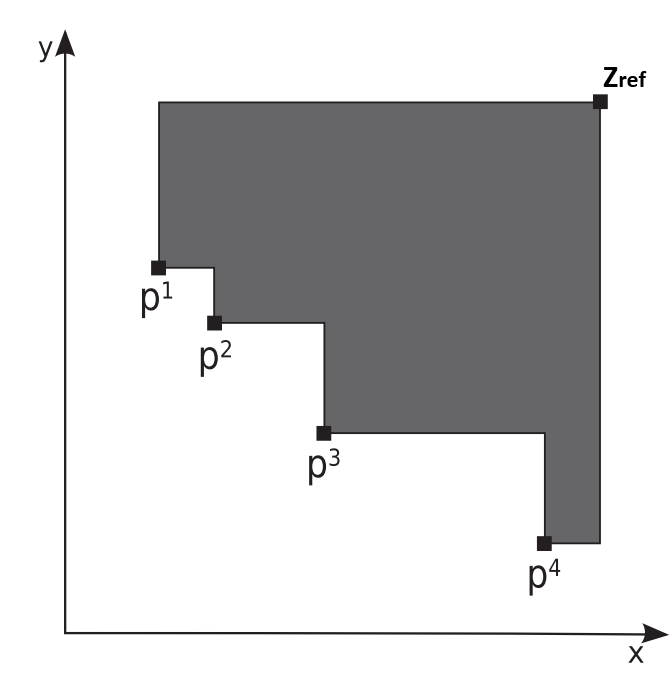
\includegraphics[width=0.6\textwidth]{fig/th_bg/hypervolume_2d.png}
    \caption{Hypervolume indicator~\cite{Guerreiro2020}.}
    \label{fig:hypervolume_2d}
\end{figure}

Figure~\ref{fig:hypervolume_2d} shows a two-dimensional example of the hypervolume (an area) and a fixed reference point $\mathbf{z}_{\mathrm{ref}}$.



\subsubsection{Inverted generational distance.}
The \emph{inverted generational distance} (IGD) measures the mean distance from each point of a reference set $Z$ to the closest point of the
approximation set and therefore requires a reference front, which is normally unavailable for real-world black-box problems~\cite{Cai2020A}. IGD is
furthermore not Pareto compliant: a set that dominates another can receive a worse indicator value~\cite{Cai2020A}. The modified variant IGD$^+$
removes this defect by replacing the Euclidean distance with a dominance-aware distance that only penalizes those objective components in which the
approximation set is actually worse than the reference point~\cite{Ishibuchi2015Modified}.

Figure~\ref{fig:igd_igdplus} illustrates the difference between the
distance calculations for a two-objective minimization problem. Although
solution $\mathbf{a}$ dominates solution $\mathbf{b}$, its Euclidean
distance from the reference point $\mathbf{z}$ is larger. Thus, IGD can
prefer $\mathbf{b}$ over $\mathbf{a}$. In contrast, IGD$^+$ measures the
distance from $\mathbf{z}$ to the region dominated by each solution.
Consequently, the distance for $\mathbf{a}$ is no greater than that for
$\mathbf{b}$.

\begin{figure}[H]
    \centering
    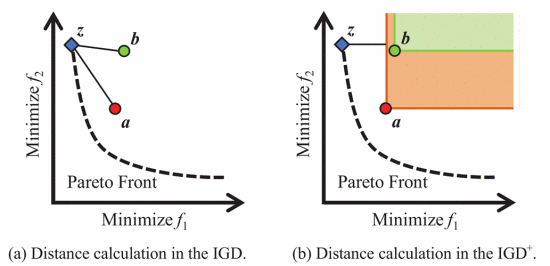
\includegraphics[width=0.9\textwidth]{fig/th_bg/igd_vs_igd_plus.png}
    \caption{Distance calculation for IGD and IGD$^+$ in a
    two-objective minimization problem. Reproduced from
    Fig.~3 of~\cite{Ishibuchi2016Sensitivity}.}
    \label{fig:igd_igdplus}
\end{figure}

\begin{equation}
    \label{eq:igd_plus}
    \begin{gathered}
        \mathrm{IGD}^{+}(A, Z) =
        \frac{1}{|Z|} \sum_{\mathbf{z} \in Z}
        \min_{\mathbf{a} \in A}
        \sqrt{ \sum_{i=1}^{k} \bigl( \max\{\, a_i - z_i,\, 0 \,\} \bigr)^{2} },
        \qquad \mathrm{IGD}^{+}(A, Z) \in \left\{ r \in \mathbb{R} \mid r \ge 0 \right\},
        \\[4pt]
        A,\, Z \subset \mathbb{R}^{k},
        \quad
        0 < |A| < \infty,
        \quad
        0 < |Z| < \infty,
        \quad
        k \in \left\{ n \in \mathbb{Z} \mid n \ge 1 \right\},
        \\[2pt]
        \mathbf{a} = (a_1,\ldots,a_k),
        \quad
        \mathbf{z} = (z_1,\ldots,z_k),
        \quad
        \forall\, \mathbf{a} \in A,
        \quad
        \forall\, \mathbf{z} \in Z.
    \end{gathered}
\end{equation}

In Equation~\eqref{eq:igd_plus}, $A$ denotes the approximation set under
evaluation, while $a_i$ and $z_i$ denote the $i$-th objective values of an
approximation point and a reference point, respectively. Lower values indicate
better approximation quality, and IGD$^+$ is weakly Pareto
compliant~\cite{Ishibuchi2015Modified}. Because the true Pareto front of the
gripper design problem is unknown, the reference set $Z$ is constructed as the
non-dominated union of the fronts of all compared runs~\cite{Cai2020A}. IGD$^+$
is therefore a \emph{relative} measure: it quantifies how well an individual run
approximates the best front jointly attainable by the whole set of runs, and it
is optimistically biased in favor of those runs that contribute many points to
$Z$~\cite{Cai2020A}.

% \subsubsection{Stochasticity, Seeding and Statistical Comparison}
% \label{subsubsec:stochasticity_and_statistics}

% Evolutionary algorithms and Bayesian optimization are both stochastic procedures~\cite{L'opez-Ib'anez2021Reproducibility, Wang2020IOHanalyzer}. Initial
% populations, variation operators and initial designs of experiments depend on pseudo-random numbers, so a single run of an algorithm on a given
% problem yields only one realisation of a random variable. Conclusions drawn from single runs are consequently not reproducible and may reflect chance
% rather than algorithm quality~\cite{Vermetten2022Analyzing}.

% Two measures address this issue. First, every run is initialised with an explicitly recorded random seed, which makes individual experiments
% reproducible and allows algorithms to be compared on identical initial conditions~\cite{L'opez-Ib'anez2021Reproducibility}. Second, each algorithm and
% problem combination is executed for a number of independent repetitions, and the resulting indicator values are reported through descriptive
% statistics such as median and interquartile range rather than a single best observed value~\cite{L' Lopez-Ib'anez2021Reproducibility}. Since indicator
% distributions are typically neither normal nor homoscedastic, non-parametric procedures are preferred for the statistical
% assessment~\cite{Latorre2020A}.

\subsection{Reference-Direction Generation}
\label{sec:reference_direction_generation}

Reference directions specify target regions in objective space and are used
by algorithms such as NSGA-III and MOEA/D to distribute their search.
Two generation methods available in \texttt{pymoo} are Das--Dennis and
energy-based generation~\cite{pymoo}.
The Das--Dennis method constructs a regular grid on the unit simplex.
For $m$ objectives and $p$ partitions, the number of directions $N$ is
\begin{equation}
    \label{eq:binom_count}
    \begin{gathered}
        N = \binom{p+m-1}{m-1},
        \\[4pt]
        p,\, m \in \left\{ n \in \mathbb{Z} \mid n \ge 1 \right\},
        \quad
        N \in \left\{ n \in \mathbb{Z} \mid n \ge 1 \right\}.
    \end{gathered}
\end{equation}
This construction is deterministic, but the direction count grows
combinatorially with the objective count for a fixed partition setting.
It also restricts the available direction counts to those produced by
the grid construction.~\cite{pymoo,das_dennis}

Energy-based generation distributes a prescribed number of points on the
unit simplex by minimizing a repulsive energy function. Unlike Das--Dennis,
it permits direct specification of the number of directions, making it useful
when a fixed reference-set size is required in higher-dimensional objective
spaces.~\cite{pymoo,ref_dirs_energy}
%-------------------------------------------------------------------
\section{Multi-Objective Evolutionary Algorithms}
\label{subsec:moea}

The candidate algorithms introduced in this section are all members of the multi-objective evolutionary algorithm (MOEA) family. Each follows the
general EA loop described in Section~\ref{subsubsec:evolutionary_algorithms} but differs in how it guides selection toward a well-distributed
approximation of the Pareto front. Brief introductions to each algorithm are given below.

\subsection{NSGA-II}
\label{subsubsec:nsga2}

The Non-dominated Sorting Genetic Algorithm II (NSGA-II) is among the most widely adopted MOEAs. Its selection mechanism is based on two criteria
applied in sequence. First, the entire population is sorted into non-domination ranks, so that all non-dominated solutions receive rank 1, they are
removed, and the process repeats until every individual has a rank. Second, within the same rank, solutions are ordered by \emph{crowding distance}, a
density estimate that measures how isolated a solution is from its neighbors in the objective space. Solutions with a higher crowding distance are
preferred, encouraging spread along the Pareto front. NSGA-II uses an elitist strategy in which the combined parent and offspring population of size
$2N$ is truncated to $N$ using these two criteria. Its computational complexity per generation is $\mathcal{O}(kN^2)$, where $k$ is the number of
objectives and $N$ is the population size.~\cite{nsga2}

\subsection{NSGA-III}
\label{subsubsec:nsga3}

NSGA-III extends NSGA-II to problems with four or more objectives (many-objective problems), where crowding distance becomes an unreliable diversity
measure. Instead of crowding distance, NSGA-III uses a set of structured \emph{reference points} distributed uniformly on a normalized hyperplane in
the objective space. Solutions are associated with their closest reference point, and selection preference is given to solutions that are associated
with under-represented reference points and lie closest to their reference line. This mechanism explicitly promotes diversity across the objective
space and has been shown to outperform NSGA-II on problems with four or more objectives.~\cite{nsga3}

\subsection{MOEA/D}
\label{subsubsec:moead}

MOEA/D (Multi-Objective Evolutionary Algorithm based on Decomposition) takes a fundamentally different approach from Pareto-ranking methods. The
multi-objective problem is decomposed into $N$ scalar subproblems using a set of evenly distributed weight vectors and an aggregation function such as
the weighted Chebyshev scalarization. Each subproblem is optimized simultaneously, with solutions sharing information within a defined neighborhood
of weight vectors. This neighborhood-based collaborative search makes MOEA/D computationally efficient and well suited to problems where the Pareto
front has a regular structure. Its complexity per generation is lower than NSGA-II, as it avoids global non-dominated sorting.~\cite{moead, pymoo}

\subsection{SMS-EMOA}
\label{subsubsec:smsemoa}

The S-Metric Selection Evolutionary Multi-Objective Algorithm (SMS-EMOA) uses the hypervolume indicator directly as its selection criterion. It
operates as a steady-state algorithm, so that at each step a single offspring is generated, added to the population, and the individual that
contributes the least to the population hypervolume is removed. This ensures that the population converges toward solutions that maximize the
dominated hypervolume with respect to a reference point. SMS-EMOA is particularly well suited to problems where solution quality is to be measured by
the hypervolume indicator, as its selection pressure is directly aligned with that metric.~\cite{smsemoa}

\subsection{CMOPSO}
\label{subsubsec:cmopso}

The Competitive Multi-Objective Particle Swarm Optimizer (CMOPSO) adapts the particle swarm optimization (PSO) framework to the multi-objective
setting. In standard PSO, each particle moves through the decision space guided by its personal best position and a global best position. CMOPSO
introduces a competitive mechanism in which particles compete in pairs within the swarm, and the losing particle updates its velocity by learning from
the winning particle rather than from a fixed global best. An external archive of non-dominated solutions is maintained to provide guidance and
preserve diversity across the Pareto front. This competitive selection strategy avoids premature convergence to a single region of the Pareto front
and has been shown to achieve fast convergence while remaining competitive with dominance-based MOEAs on standard benchmark problems.~\cite{cmopso}


%-------------------------------------------------------------------

% Suction Cup Grippers
\nomenclature{$F_{\mathrm{hold}}$}{Holding force}
\nomenclature{$\Delta p$}{Pressure difference}
\nomenclature{$p_{\mathrm{atm}}$}{Atmospheric pressure}
\nomenclature{$A_{\mathrm{seal}}$}{Effective sealed area}
\nomenclature{$S$}{Safety factor}

% Grasp Diversity
\nomenclature{$D_{\mathrm{pos}}$}{Normalized spatial diversity}
\nomenclature{$D_{\mathrm{rot}}$}{Normalized orientational diversity}
\nomenclature{$d_{\mathrm{geo}}$}{Geodesic distance on $SO(3)$}
\nomenclature{$SO(3)$}{Special orthogonal group of 3D rotations}

% Multi-Objective Optimization
\nomenclature{$\mathbf{x}$}{Decision variable vector}
\nomenclature{$\mathcal{X}$}{Feasible decision space}
\nomenclature{$\mathbf{f}(\mathbf{x})$}{Objective function vector}
\nomenclature{$f_i(\mathbf{x})$}{Individual objective function}

% Pareto Optimality
\nomenclature{$\mathbf{x}^{(a)} \prec \mathbf{x}^{(b)}$}{Dominance relation (solution $a$ dominates $b$)}

% Gaussian Process Surrogates
\nomenclature{$\mathcal{GP}$}{Gaussian process}
\nomenclature{$\kappa(\mathbf{x}, \mathbf{x}')$}{Covariance/kernel function}
\nomenclature{$\mathcal{D}$}{Observed data set}
\nomenclature{$\mu(\mathbf{x})$}{Predictive mean}
\nomenclature{$\sigma^2(\mathbf{x})$}{Predictive variance}

% Acquisition Functions
\nomenclature{$\alpha_{\mathrm{EI}}(\mathbf{x})$}{Expected improvement acquisition}
\nomenclature{$f_{\min}$}{Best observed objective value}

% Performance Indicators
\nomenclature{$\mathrm{HV}(A, \mathbf{z}_{\mathrm{ref}})$}{Hypervolume indicator}
\nomenclature{$\mathbf{z}_{\mathrm{ref}}$}{Hypervolume reference point}